\subsection{Polytopes}
\label{sec:polytopes}

%We can also use Hypersliceplorer to examine polytopes. 
Polytopes are the
generalization of polygons and polyhedra to any number of dimensions.
Naturally, in more than three dimensions we have no way of viewing these
objects directly. Common ways to view them is either through
projections, such as the Schlegel diagram~\cite{Sommerville:1929}, or as a
graph representation, like the Hasse diagram~\cite{Battista:1988}. Projection
methods do not accurately show distances or angles. These must be distorted to
show a multi-dimensional object in two or three dimensions. Network diagrams do
not necessarily show symmetries or structure unless care is taken during
layout.

\begin{figure} 
  \centering
  \begin{subfigure}[b]{0.45\linewidth}
    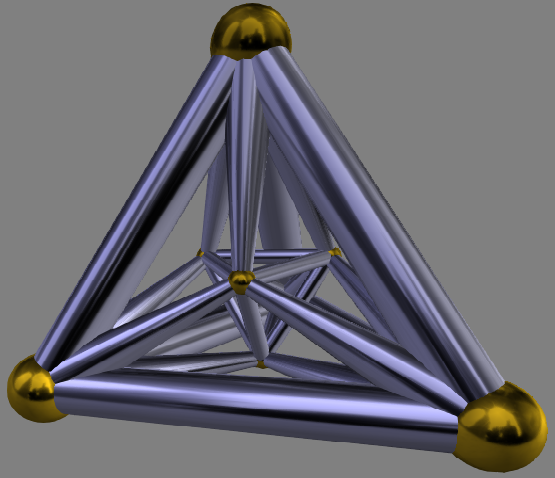
\includegraphics[width=\textwidth]{hsp_16cell-schlegel.png}
    \caption{Schlegel diagram: 16-cell (4D) generated using Stella4D~\cite{Stella4D}}
    \label{fig:ortho:schlegel} 
  \end{subfigure} 
  ~
  \begin{subfigure}[b]{0.45\linewidth}
    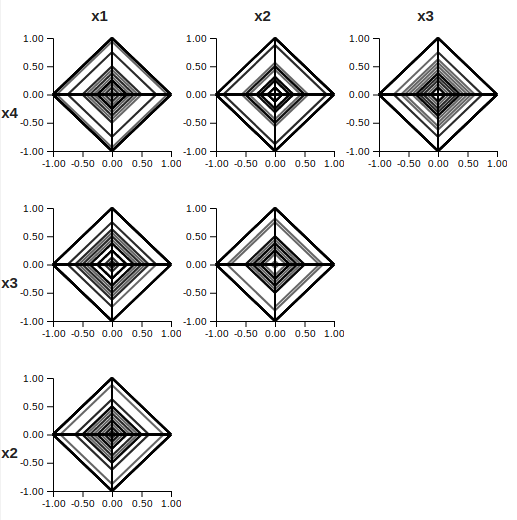
\includegraphics[width=\textwidth]{hsp_16cell-global.png}
    \caption{Hypersliceplorer: 16-cell (4D)}
    \label{fig:ortho:4} 
  \end{subfigure}
  \\
  \begin{subfigure}[b]{0.45\linewidth}
    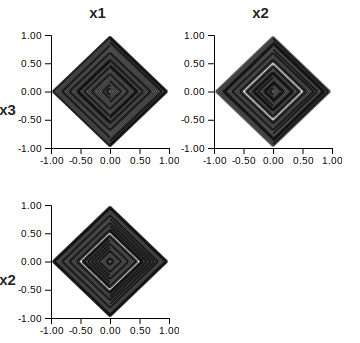
\includegraphics[width=\textwidth]{hsp_octo-global.png}
    \caption{Hypersliceplorer: Octahedron (3D)}
    \label{fig:ortho:3} 
  \end{subfigure}
  ~
  \begin{subfigure}[b]{0.45\linewidth}
    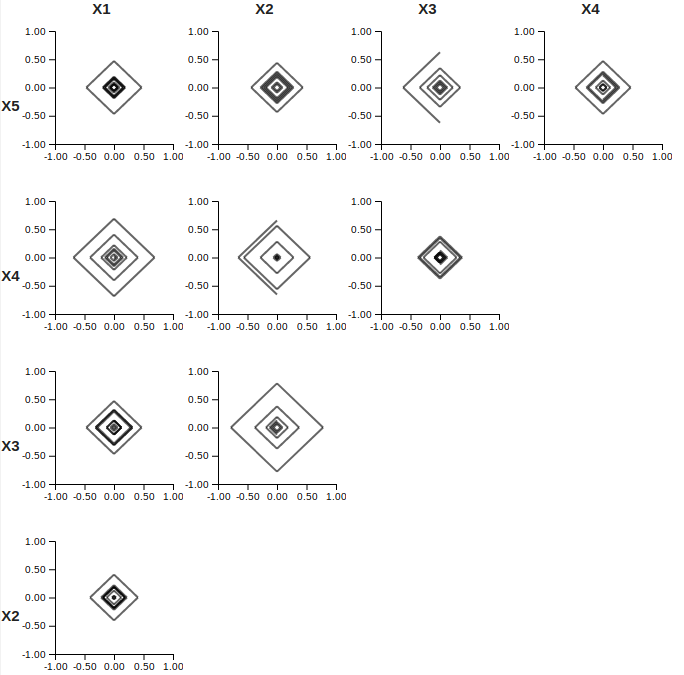
\includegraphics[width=\textwidth]{hsp_5ortho-global.png}
    \caption{Hypersliceplorer: 5-orthoplex (5D)}
    \label{fig:ortho:5} 
  \end{subfigure} 
  \caption[Views of regular polytopes]{%
    This figure shows the 16-cell, the 4-dimensional regular orthoplex (4D 
    version of
    an octahedron) as (\subref{fig:ortho:schlegel}) a Schlegel diagram and
    (\subref{fig:ortho:4}) the Hypersliceplorer view. The Hypersliceplorer
    view shows the outside shape of the figure and the repeating structure.
    We can also see the repeating structure in the 3D (\subref{fig:ortho:3})
    and 5D (\subref{fig:ortho:5}) views.
  } 
  \label{fig:orthos} 
\end{figure}

As an alternative, we can slice these polytopes and examine the slices.
Regular polytopes have well-studied structure and symmetries so I use these as
verification examples. I examine these with Hypersliceplorer and see if the
structure matches reality.  For example, in \autoref{fig:orthos} I show a
16-cell which is the four-dimensional version of an octahedron in both
Hypersliceplorer (\autoref{fig:ortho:4}) and as a Schlegel diagram (\autoref{fig:ortho:schlegel})
using the Stella4D software~\cite{Stella4D}. The
Schlegel diagram picks a face of the 16-cell and projects the remaining
structure inside it. In this case, each face of the 16-cell is a simplex. From
the Schlegel diagram it is difficult to see that the dual of the 16-cell is the
hypercube (i.e.\ each vertex of the hypercube corresponds to a face of the 16-cell and vice
versa). However, in Hypersliceplorer this property is clear from looking at the
cross sections. We can see that each cross section looks like a rotated cube
which comes from the dual property. In addition, we can see the simplical faces
from the horizontal and vertical lines in the view. These result from intersections of the
2D slice with a face of the 16-cell directly.

Further, Hypersliceplorer allows us the visualization 3D or 5D analogs of the 16-cell (the octahedron in 3D, \autoref{fig:ortho:3}, as well as the 5-orthoplex in 5D, \autoref{fig:ortho:5}). The Schlegel diagrams cannot be scaled to higher dimensions.

We can also look at other regular polytopes in the same fashion. 
\autoref{fig:cubes} shows a hypercube in 3-, 4-, and 5-dimensions. From these
plots we can clearly see the generalization of the square, to the cube, to
higher dimensions. One of the advantages of my method is that I do not need
to choose a face to project into. For example, with a discretized hypersphere,
there are many faces. We can see in \autoref{fig:spheres} the regular cross
section of a sphere as well. 

\begin{figure} 
  \centering
  \begin{subfigure}[b]{0.3\linewidth}
    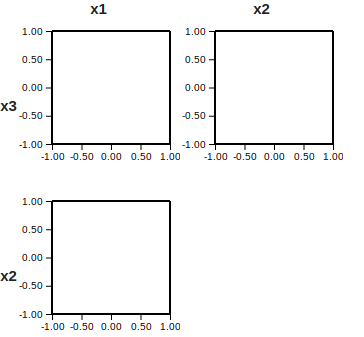
\includegraphics[width=\textwidth]{hsp_3cube.png}
    \caption{3D}
    \label{fig:cubes:3d} 
  \end{subfigure} 
  ~
  \begin{subfigure}[b]{0.3\linewidth}
    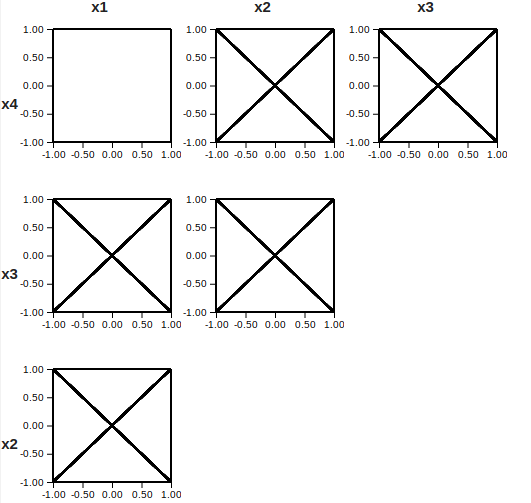
\includegraphics[width=\textwidth]{hsp_4cube.png}
    \caption{4D}
    \label{fig:cubes:4d} 
  \end{subfigure}
  ~
  \begin{subfigure}[b]{0.3\linewidth}
    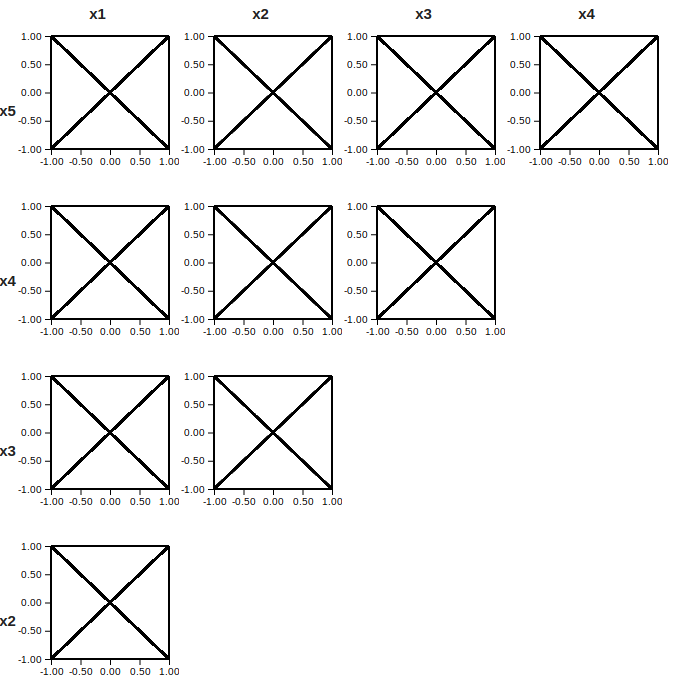
\includegraphics[width=\textwidth]{hsp_5cube.png}
    \caption{5D}
    \label{fig:cubes:5d} 
  \end{subfigure}
  \caption[3-, 4-, and 5-dimensional hypercubes.]{%
    3-, 4-, and 5-dimensional hypercubes. We can see the regular structure
    in the cubes. The cross sections are all the same size since the cube
    is oriented to the axes. The cross lines in the plots are due to the 
    simplical mesh.
  } 
  \label{fig:cubes} 
\end{figure}

\begin{figure} 
  \centering
  \begin{subfigure}[b]{0.3\linewidth}
    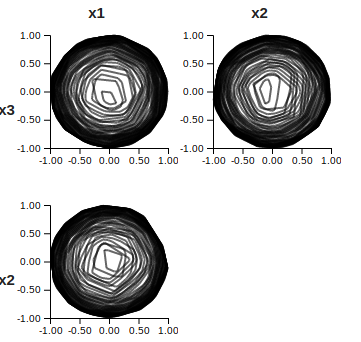
\includegraphics[width=\textwidth]{hsp_sphere_3d.png}
    \caption{3D}
    \label{fig:spheres:3d} 
  \end{subfigure} 
  ~
  \begin{subfigure}[b]{0.3\linewidth}
    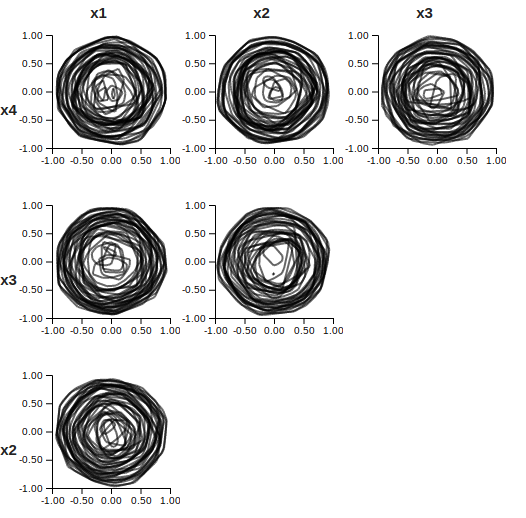
\includegraphics[width=\textwidth]{hsp_sphere_4d.png}
    \caption{4D}
    \label{fig:spheres:4d} 
  \end{subfigure}
  ~
  \begin{subfigure}[b]{0.3\linewidth}
    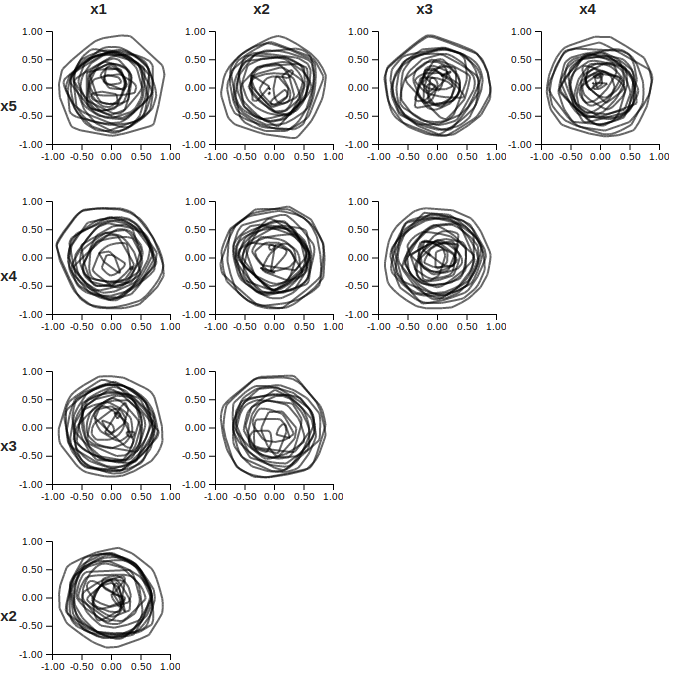
\includegraphics[width=\textwidth]{hsp_sphere_5d.png}
    \caption{5D}
    \label{fig:spheres:5d} 
  \end{subfigure}
  \caption[3-, 4-, and 5-dimensional hyperspheres.]{%
    3-, 4-, and 5-dimensional hyperspheres. We can see the concentric rings
    from slicing the sphere at different points. The irregularity of the
    slices is due to sampling.
  } 
  \label{fig:spheres} 
\end{figure}


